\chapter{On the Transferability of Convolutional Networks}
\label{ch:tl_natural_to_non_natural}

\begin{remark}{Contributions and Outline} 
	We now present a first study that characterizes the Transfer Learning (TL) properties of convolutional neural networks that come as pre-trained on the ImageNet dataset. We thoroughly investigate whether popular neural networks that have obtained state of the art results on this benchmark of natural images can perform equally well once used on non-natural datasets. Specifically, we explore whether it is possible to tackle three different target tasks $\mathcal{T_T}$ that come in the form of art classification problems. We study the effects of different TL training approaches (off-the-shelf classification vs. fine-tuning), and explore whether it is possible to improve the TL performance of the considered pre-trained networks by allowing these models to have access to source domains $\mathcal{D}_S$ other than the ImageNet dataset exclusively. The chapter is structured as follows: we start by providing the reader with some background information in Sec. \ref{sec:ch_4_introduction}. In Sec. \ref{sec:ch_4_methods} we present a brief theoretical reminder of the field of TL, a description of the datasets that we have used, and the methodological details about the experiments that we have performed. In Sec. \ref{sec:ch_4_results} we present and discuss our results. A summary of the main contributions of this chapter is finally presented in Sec. \ref{sec:ch_4_conclusion}.

\vspace{5mm}
\textit{This chapter is based on the publication \citet{sabatelli2018deep}.}
\end{remark}



\iffalse
% ---- Section 1 ----
\section{Introduction and Related Work}
\label{sec:introduction}


In this work we explore whether the TL paradigm can be successfully applied to three different art classification problems. We use four neural architectures that have obtained strong results on the ImageNet challenge in recent years and we investigate their performance when it comes to attributing the \textit{authorship} to different artworks, recognizing the \textit{material} which has been used by the artists in their creations, and identifying the \textit{artistic category} these artworks fall into. We do so by comparing two possible approaches that can be used to tackle the different classification tasks. The first one, known as off-the-shelf classification \cite{razavian2014cnn}, simply retrieves the features that were learned by the networks on other datasets and uses them as input for a new classifier. In this scenario the weights of the model do not change during the training phase, and the final, top-layer classifier is the only component of the architecture which is actually trained. This changes in our second explored approach, known as fine-tuning, where the weights of the original network are ``unfrozen'' and the neural architectures are trained together with the final classifier. 

\citet{kornblith2018better} have shown the benefits that this particular pre-training approach has. In particular, DCNNs which have been trained on the ImageNet challenge typically lead to superior results when compared to the same architectures trained from scratch. However, this is not necessarily beneficial and in some cases networks that are randomly initialized are able to achieve the same performance as ImageNet pre-trained models. However, none of the results presented in \cite{kornblith2018better} report experiments on datasets containing heritage objects, it is thus still an open question how such pre-trained DCNNs would perform in such a classification scenario. In the rest of this chapter we report results that extensively study the performance of such neural networks; at the same time we also assess whether better TL performance can be obtained when using neural networks that, in addition to the ImageNet dataset, have additionally been pre-trained on a large artistic collection.  

\fi

\section{A First Empirical Study}
\label{sec:ch_4_introduction}

In the first part of this thesis, we have seen that convolutional neural networks have become a crucial component in today's machine learning toolbox. Thanks to their ability to automatically learn relevant features, these neural networks can successfully be used for tackling both supervised learning problems, as well as reinforcement learning ones. Specifically, as reviewed in Chapter \ref{ch:transfer_learning}, thanks to the field of deep transfer learning it is now possible to find a broad range of successful applications that see the usage of convolutional networks even outside the domain these networks were originally developed for, namely natural images \cite{kornblith2018better}. Despite many successfull examples, there still are some domains for which their applicability, and therefore potential transfer learning properties, have not been explored. A promising research field in this sense is that of \textcolor{RoyalBlue}{Digital Heritage} \cite{parry2005digital}. Due to a growing and rapid process of digitization, museums have started to digitize large parts of their cultural heritage collections, leading to the creation of several digital open datasets \cite{allen2000collaboration, mensink2014rijksmuseum}. The images constituting these datasets are mostly matched with descriptive metadata, which, as presented by \citet{mensink2014rijksmuseum}, can be used for defining a set of challenging machine learning tasks. However, the image samples in these datasets are very different in terms of quantity, size, and resolution from the images that typically constitute popular computer vision benchmarks; therefore, the computer vision potential of convolutional networks in this domain is largely unknown. In this chapter, we address this research question and present a first, thorough, empirical study that explores the potential that convolutional neural networks have to offer when transferred to the artistic domain. The next section moves towards providing the reader with a brief formal reminder of TL. We then introduce the three classification problems that are considered in our study, together with a brief description of the datasets. Finally, we present the neural architectures that we have used for the experiments. 

\section{Methodology}
\label{sec:ch_4_methods}
\subsection{Transfer Learning}
\label{subsec:tl}

As seen in Chapter \ref{ch:supervised_learning}, a supervised learning (SL) problem can be identified by three elements: an input space ${\cal X}_T$, an output space ${\cal Y}_T$, and a probability distribution $p_T(x,y)$ defined over ${\cal X}_T\times {\cal Y}_T$ (where $T$ stands for 'target', as this is the main problem we would like to solve). The goal of SL is then to build a function $f:{\cal X}_T\rightarrow{\cal Y}_T$ that minimizes the expectation over $p_T(x,y)$ of a given loss function $\ell$ assessing the predictions made by $f$:
\begin{equation}\label{loss}
  E_{(x,y)\sim p_t(x,y)} \{\ell(y,f(x))\},
\end{equation}
where the only information available to build this function is a learning sample of input-output pairs $LS_T=\{(x_i,y_i)|i=1,\ldots,N_T\}$ drawn independently from $p_T(x,y)$. As introduced in Chapter \ref{ch:transfer_learning}, in the general transfer learning setting, one assumes that an additional dataset $LS_S$, called the source data, is available that corresponds to a different, but related, SL problem. More formally, the source SL problem is assumed to be defined through a triplet $({\cal X}_S,{\cal Y}_S,p_S(x,y))$, where at least either ${\cal X}_S\neq {\cal X}_T$, ${\cal Y}_S\neq {\cal Y}_T$, or $p_S\neq p_T$. The goal of TL is then to exploit the source data $LS_S$ together with the target data $LS_T$ to potentially find a better model $f$ in terms of the expected loss (\ref{loss}) than when only $LS_T$ is used for training this model.
We have seen that depending on the availability of labels in the target and source data and on how the source and target problems differ, one can distinguish different TL settings (see Sec. \ref{sec:tl_general_framework} of Chapter \ref{ch:transfer_learning}). In what follows, we assume that labels are available in both the source and target data and that the input spaces ${\cal X}_T$ and ${\cal X}_S$, that both correspond to color images, match. However, output spaces and joint distributions will differ between the source and target problems, as they will correspond to different classification problems (ImageNet object recognition versus art classification tasks). We, therefore, consider the inductive transfer learning setup and assume that information between the source and target problems is exchanged in the form of a neural network that comes as pre-trained on the source data. 

\subsection{Datasets and Target Tasks $\mathcal{T}_T$}
\label{subsec:datasets}

For our experiments, we use two datasets that come from two different heritage collections. The first one contains the largest number of samples and comes from the Rijksmuseum in Amsterdam\footnote{\url{https://staff.fnwi.uva.nl/t.e.j.mensink/uva12/rijks/}}. On the other hand, our second `Antwerp' dataset is much smaller. This dataset presents a random sample that is available as open data from a larger heritage repository: DAMS (Digital Asset Management System)\footnote{\url{https://dams.antwerpen.be/}}. This repository can be searched manually via the web interface or queried via a Linked Open Data API. It aggregates the digital collections of the foremost GLAM institutions  (Galleries, Libraries, Archives, Museums) in the city of Antwerp in Belgium. Thus, this dataset presents a varied and representative sample of the sort of heritage data nowadays being collected at the level of individual cities across the globe. While it is much smaller, its coverage of cultural production is similar to that of the Rijksmuseum dataset and presents an ideal testing ground for the transfer learning task under scrutiny here. Both image datasets come with metadata encoded in the Dublin Core metadata standard \cite{weibel1998dublin}. We selected three well-understood classification problems:
\begin{itemize}
	\item \textcolor{RoyalBlue}{Material classification:} which consists in identifying the material the different heritage objects are made of (e.g., paper, gold, porcelain, ...); 
	\item \textcolor{RoyalBlue}{Type classification:} in which the neural networks have to classify in which artistic category the samples fall into (e.g., print, sculpture, drawing, ...);
	\item \textcolor{RoyalBlue}{Artist classification:} where the main goal is to match each sample of the dataset with its creator.
\end{itemize}

As the goal is to tackle these classification problems through TL, we will refer to them as $\mathcal{T}_T$ \circled{1}, $\mathcal{T}_T$ \circled{2} and $\mathcal{T}_T$ \circled{3} respectively. As reported in Table \ref{table:dataset_overview} we can see that the Rijksmuseum collection is the dataset with the largest amount of samples per target task ($N_t$) and the highest amount of labels to classify ($Q_t$). Furthermore, it is also worth noting that there was no metadata available when it comes to the first classification task for the Antwerp dataset (as marked by the $-$ symbol), and that there are some common labels between the two heritage collections when it comes to the classification of types ($\mathcal{T}_T$ \circled{2}). A visualization reporting some of the images that are present in both datasets is shown in Fig. \ref{fig:datasets}.


\begin{table}[ht!]
\scriptsize
\centering
\caption{An overview of the two datasets that are used in our experiments. For each heritage collection we report with $N_t$ the amount of samples constituting the datasets and with $Q_t$ the number of labels. Lastly, we also report if there are common labels between the two heritage collections.}
\begin{tabular}{c|c|c|c|c} 
	\hline
	$\mathcal{T}_T$ & Dataset & \textbf{$N_t$} & \textbf{$Q_t$} & $\%$ of overlap \\\hline \hline
        Material \circled{1} & Rijksmuseum  & $110,668$ & $206$ &  $\varnothing$ \\ 
         & Antwerp & $-$ & $-$    \\
        Type \circled{2} & Rijksmuseum  & $112,012$ & $1,054$   \\
         & Antwerp & $23,797$ & $920$ & $\approx 15\%$ \\
        Artist \circled{3} & Rijksmuseum & $82,018$ & $1,196$  & $\varnothing$ \\ 
         & Antwerp  & $18,656$ & $903$ \\        
	\hline
\end{tabular}
\label{table:dataset_overview}
\end{table}   



\begin{figure}
\centering
  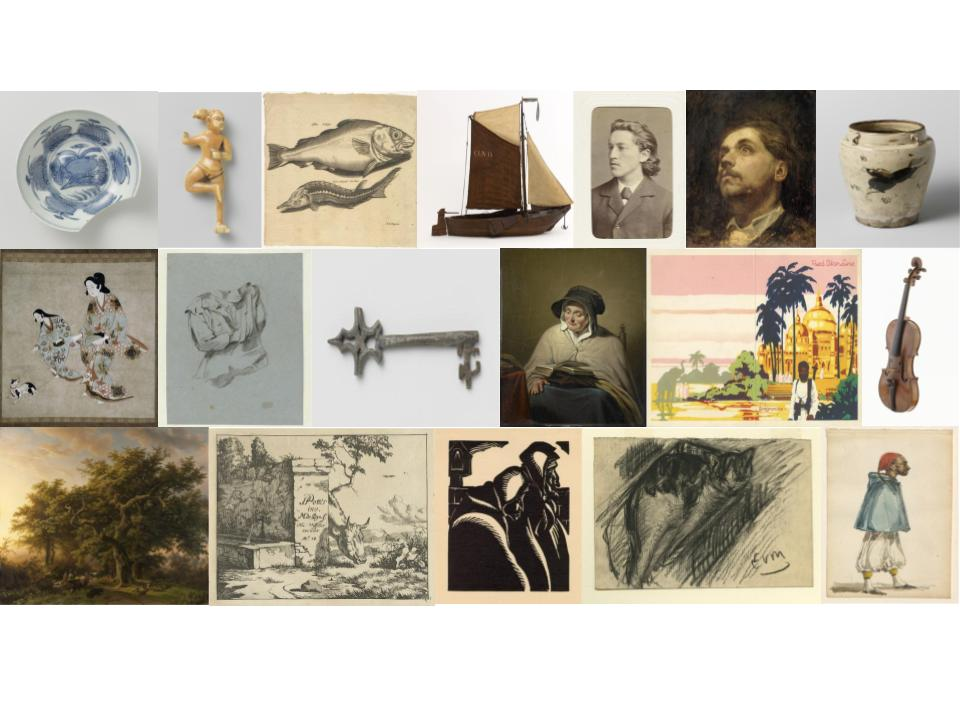
\includegraphics[width=10cm]{./Images/Chapter04/datasets.jpg}\vspace{-1cm}
  \caption{A visualization of the images that are used for our experiments. It is possible to see how the samples range from images representing plates made of porcelain to violins, and from Japanese artworks to a more simple picture of a key.}
  \label{fig:datasets}
\end{figure}

We use $80\%$ of the datasets for training while the remaining $2 \times 10\%$ is used for validation and testing respectively. Furthermore, we ensure that only classes which occur at least once in all the splits are used for our experiments. Naturally, in order to keep all comparisons fair between neural architectures and different TL approaches, all experiments have been performed on the exact same data splits.

\subsection{Convolutional Networks and Training Approaches}
\label{subsec: neural_nets}

For our experiments, we use four pre-trained convolutional networks that were reviewed in Chapter \ref{ch:supervised_learning} and that have all obtained state-of-the-art results on the ImageNet classification challenge. These neural architectures are VGG19 \cite{simonyan2014very}, Inception-V3 \cite{szegedy2016rethinking}, Xception \cite{chollet2016xception} and ResNet50 \cite{xie2017aggregated}. We use the implementations of the networks that are provided by the \texttt{Keras} Deep Learning library \cite{chollet2015keras} together with their appropriate \texttt{Tensorflow} weights \cite{abadi2016tensorflow} that come from the \texttt{Keras} official repository as well. Since all architectures have been built in order to deal with the ImageNet dataset, we replace the final classification layer of each network with a new one. This final layer simply consists of a new softmax output, with as many neurons as there are classes to classify, which follows a 2D global average pooling operation. We rely on this dimensionality reduction step because we do not add any fully connected layers between the last convolution layer and the softmax output. Hence, in this way, we are able to obtain a feature vector, $\mathscr{X}$, out of the rectified activation feature maps of the network that can be properly classified. Since all experiments are treated as a multi-class classification problem, all networks minimize the categorical crossentropy loss function. We investigate the potential of the TL approaches that were reviewed in Chapter \ref{ch:transfer_learning}, which, as a reminder, are: the off-the-shelf classification approach, which only trains the final softmax classifier on $\mathscr{X}$ retrieved after performing one forward pass of the image through the network and the fine-tuning approach, which differs from the previous one by the fact that together with the final softmax output the entire network is trained as well. 
From now on, we refer to the networks trained with the off-the-shelf classification approach as $\theta^{-}_{i}$, while to the fine-tuned networks simply as $\theta_{i}$, where $i$ stands for the source task $\mathcal{T}_S$ these models have been trained on, namely the ImageNet ($i$) dataset. In order to maximize the performance of all models, we follow some of the recommendations presented by \citet{masters2018revisiting} and train the networks with a relatively small batch size of $32$ samples. We do not perform any data augmentation operations besides a standard pixel normalization to the $[0, 1]$ range and a re-scaling operation that resizes the images to the input size that the different models require. Regarding the stochastic optimization procedures of the different classifiers, we use two different optimizers, that after preliminary experiments, turned out to be the best-performing ones. For the off-the-shelf approach we use the RMSprop optimizer \cite{tieleman2012lecture} which has been initialized with its default hyperparameters (learning rate = $0.001$, a momentum value $\rho = 0.9$ and $\epsilon =1e-08$). On the other hand, when we fine-tune the models, we use the standard Stochastic Gradient Descent (SGD) algorithm with the same learning rate, $0.001$, and a Nesterov Momentum value \cite{nesterov1983method} set to $0.9$.
Training has been controlled by the early stopping method \cite{caruana2001overfitting} which interrupted training as soon as the validation loss did not decrease for $7$ epochs in a row. The model which is then used on the testing set is the one that obtained the smallest validation loss while training.

% END METHODS
%==================================================================================================================
% BEGIN RESULTS

\section{Results}
\label{sec:ch_4_results}

Our experimental results are divided into two sections, depending on which kind of dataset has been used. We first report the results that we have obtained when using architectures that were pre-trained on the ImageNet dataset only and aimed to tackle the three classification tasks of the Rijksmuseum dataset that were presented in Section \ref{subsec:datasets}. We report these results in Section \ref{subsec: natural_to_art} where we explore the benefits of using the ImageNet dataset as source domain $\mathcal{D}_S$ only, and how well such pre-trained models generalize when it comes to the artistic target domain. We then present the results from classifying the Antwerp dataset, using models that are both pre-trained on the ImageNet dataset and on the Rijksmuseum collection in Section \ref{subsec: from_one_to_another}. We investigate whether these neural architectures, which have already been trained to tackle art classification problems before, perform better than those trained on the ImageNet dataset only.    
All results show comparisons between the off-the-shelf classification approach and the fine-tuning scenario. In addition to that, in order to establish the potential benefits that TL from ImageNet has over training a model from scratch, we also report the results that have been obtained when training a network with weights that have been initially sampled from a He-Uniform distribution \cite{he2015delving}. Since we take advantage of the work presented by \citet{bidoiadeep} we use the Inception-V3 architecture. We refer to it in all figures as Scratch-V3 and always visualize it with a solid orange line. Fig. \ref{fig:rijks_material} and Fig. \ref{fig:type_and_artist} report the performance in terms of accuracy ($\%$) that the models have obtained on the validation sets. While the performance that the neural architectures have obtained on the final testing set are reported in Tables \ref{tab:Rijksmuseum_Dataset} and \ref{tab:Antwerpen_dataset}. 


\subsection{From Natural to Non Natural Images}
\label{subsec: natural_to_art}

The first results that we report have been obtained on $\mathcal{T}_T$ \circled{1}, namely the material classification task. We believe that this can be considered as the easiest classification task within the ones that we have introduced in Section \ref{subsec:datasets} for two main reasons: first, the number of possible classes the networks have to deal with is more than five times smaller when compared to the other two challenges; second, we also believe that this classification task is, within limits, the most similar one when compared to the original ImageNet challenge. Hence, the features that might be useful to classify the different natural images on the latter classification testbed might not be too dissimilar from the ones needed to properly recognize the material that the different samples of the Rijksmuseum collection are made of. If this were the case, we would expect a very similar performance between the off-the-shelf classification approach and the fine-tuning one. Comparing the learning curves of the two classification strategies in Fig. \ref{fig:rijks_material}, we observe that the fine-tuning approach leads to significant improvements when compared to the off-the-shelf one for three architectures out of the four tested ones. Note, however, that, in support of our hypothesis, the off-the-shelf approach can still reach high accuracy values on this problem and is also competitive with the model trained from scratch, with the crucial difference being that these models result in faster training as \textcolor{RoyalBlue}{jumpstart improvements} can be observed. This suggests that features extracted from networks pretrained on ImageNet are relevant for the target task $\mathcal{T}_T$ of material classification.

\begin{figure}[ht]
  \centering
  \begin{tikzpicture}[scale = 0.8]

\begin{axis}[
	grid style={dashed,gray},
	grid = both, 
	tick style=black,
  	xlabel=Epochs,
  	ylabel= Accuracy ($\%$),
	title=Material Classification,
	%width=1,
    	xmin=0,
    	xmax=10,
    	ymin=0.80,
    	ymax=0.95,
  	legend pos=outer north east,
]

	\addlegendentry{Xception $\theta^{i}$}
	\addlegendentry{ResNet50 $\theta^{i}$}
	\addlegendentry{InceptionV3 $\theta^{i}$}
	\addlegendentry{VGG19 $\theta^{i}$}
      	\addlegendentry{Scratch-V3 $\theta$}
      	\addlegendentry{Xception $\theta^{-}$}
      	\addlegendentry{ResNet50 $\theta^{-}$}
      	\addlegendentry{InceptionV3 $\theta^{-}$}
      	\addlegendentry{VGG19 $\theta^{-}$}


\addplot [thick, blue, mark=x] table [y=Xception, x=epochs]
{./Results/Chapter03/logs/res_1.txt};
\addplot [thick, red, mark=x] table [y=ResNet, x=epochs]{./Results/Chapter04/logs/res_1.txt};
\addplot [thick, black, mark=x] table [y=V3, x=epochs]{./Results/Chapter04/logs/res_1.txt};
\addplot [thick, green, mark=x] table [y=VGG19, x=epochs]{./Results/Chapter04/logs/res_1.txt};
\addplot [ultra thick, orange , solid] table [y=RandomV3, x=epochs]{./Results/Chapter04/logs/res_1.txt};


\addplot [ thick, blue, mark=halfcircle] table [y=Xception, x=epochs]{./Results/Chapter04/logs/res_2.txt};
\addplot [ thick, red, mark=halfcircle] table [y=ResNet, x=epochs]{./Results/Chapter04/logs/res_2.txt};
\addplot [thick, black, mark=halfcircle] table [y=V3, x=epochs]{./Results/Chapter04/logs/res_2.txt};
\addplot [thick, green, mark=halfcircle] table [y=VGG19, x=epochs]{./Results/Chapter04/logs/res_2.txt};



\end{axis}
    \end{tikzpicture}
    \caption{Comparison between the fine tuning approach ($\theta^{i}$) versus the off the shelf one ($\theta^{-}$) when classifying the material of the heritage objects of the Rijksmuseum dataset. We can observe that for three out of four neural architectures the first approach leads to significant improvements when compared to the latter one. Furthermore, we can also observe that training a randomly initialized model from scratch (solid orange line) leads to worse results than fine-tuning a network that comes as pre-trained on the ImageNet dataset.}
    \label{fig:rijks_material}
\end{figure} 


We can also observe that the ResNet50 architecture is the architecture that, when fine-tuned, performs overall best compared to the other three models. This happens despite it being the network that initially performed worse as a simple feature extractor in the off-the-shelf experiments. As reported in Table \ref{tab:Rijksmuseum_Dataset} we can see that this kind of behavior reflects itself on the separated testing set as well, where it obtained the highest testing set accuracy when fine-tuned ($92.95\%$), and the lowest one when the off-the-shelf approach was used ($86.81\%$). It is worth noting that the performance between the different neural architectures do not strongly differ between each other once they are fine-tuned, with all models performing around $\approx 92\%$ on the final testing set. Furthermore, special attention needs to be given to the VGG19 architecture, which does not seem to benefit from the fine-tuning approach as much as the other architectures do. In fact, its off-the-shelf performance on the testing set ($92.12\%$) is very similar to its fine-tuned one ($92.23\%$). This suggests that this neural architecture is the only one that, in this task, and when pre-trained on ImageNet, can successfully be used as a simple feature extractor without relying on complete retraining. 

When analyzing the performance of the different neural architectures on $\mathcal{T}_T$ \circled{2} (type classification) and $\mathcal{T}_T$ \circled{3} (artist classification), respectively the left and right plots reported in Fig. \ref{fig:type_and_artist}, we observe that on these problems the fine-tuning strategy leads to even more significant improvements when compared to what we observed in the previous experiment. The results obtained on the second task show again that the ResNet50 architecture is the architecture that leads to the worse results if the off-the-shelf approach is used (its testing set accuracy is as low as $71.23\%$), and similarly to what has been observed before, it then becomes the best performing model when fine-tuned, with a final accuracy of $91.30\%$. Differently from what has been observed in the previous experiment, the VGG19 architecture, despite being the network performing best when used as off-the-shelf feature extractor, this time performs significantly worse than when it is fine-tuned, which highlights the benefits of this latter training approach. Similar to what has been observed before, our results are again not significantly favoring any fine-tuned neural architecture, with all final accuracies being around $\approx 91\%$.

If the so far considered target tasks have highlighted the significant benefits of the fine-tuning approach over the off-the-shelf one, it is also important to note that the latter approach is still able to yield satisfying results. In fact, a final accuracy of $92.12\%$ has been obtained when using the VGG19 architecture for tackling $\mathcal{T}_T$ \circled{1}, and the same architecture reached a classification rate of $77.33\%$ on $\mathcal{T}_T$ \circled{2}. Despite the latter accuracy being very far in terms of performance from the one obtained when fine-tuning the network ($90.27\%$), these results still show that models pre-trained on ImageNet do learn particular features that can also be used for classifying the material and the type of heritage objects. In fact, \textcolor{RoyalBlue}{jumpstart improvements} were observed in Fig. \ref{fig:rijks_material} as well as in the left plot of Fig. \ref{fig:type_and_artist}. 


\begin{figure}[ht!]
  \begin{tikzpicture}[scale = 0.65]
      \begin{axis}[
	name=ax1,
      	grid style={dashed,gray},
      	grid = both, 
      	tick style=black,
	title=$\mathcal{T}_T$ \circled{2},
        xlabel=Epochs,
        ylabel= Accuracy ($\%$),
	ymin=0.65,
      ]


      \addlegendentry{Xception $\theta^{-}_{i}$}
      \addlegendentry{ResNet50 $\theta^{-}_{i}$}
      \addlegendentry{InceptionV3 $\theta^{-}_{i}$}
      \addlegendentry{VGG19 $\theta^{-}_{i}$}
	\addlegendentry{Scratch-V3 $\theta$}
	\addlegendentry{Xception $\theta_{i}$}
	\addlegendentry{ResNet50 $\theta_{i}$}
	\addlegendentry{InceptionV3 $\theta_{i}$}
	\addlegendentry{VGG19 $\theta_{i}$}

      \addplot [thick, blue, mark=diamond] table [y=Xception, x=epochs]
      {./Results/Chapter04/logs/rijksmuseum_type_challenge_only_softmax.txt};
      \addplot [thick, red, mark=diamond] table [y=ResNet, x=epochs]{./Results/Chapter04/logs/rijksmuseum_type_challenge_only_softmax.txt};
      \addplot [thick, black, mark=diamond] table [y=V3, x=epochs]{./Results/Chapter04/logs/rijksmuseum_type_challenge_only_softmax.txt};
      \addplot [thick, green, mark=diamond] table [y=VGG19, x=epochs]{./Results/Chapter04/logs/rijksmuseum_type_challenge_only_softmax.txt};
            \addplot [ultra thick, orange , solid] table [y=ScratchV3, x=epochs]{./Results/Chapter04/logs/rijksmuseum_type_challenge_full_fine_tuning.txt};

      \addplot [ thick, blue, mark=x] table [y=Xception, x=epochs]{./Results/Chapter04/logs/rijksmuseum_type_challenge_full_fine_tuning.txt};
      \addplot [ thick, red, mark=x] table [y=ResNet, x=epochs]{./Results/Chapter04/logs/rijksmuseum_type_challenge_full_fine_tuning.txt};
      \addplot [thick, black, mark=x] table [y=V3, x=epochs]{./Results/Chapter04/logs/rijksmuseum_type_challenge_full_fine_tuning.txt};
      \addplot [thick, green, mark=x] table [y=VGG19, x=epochs]{./Results/Chapter04/logs/rijksmuseum_type_challenge_full_fine_tuning.txt};

\legend{}

      \end{axis}

      \begin{axis}[
	at={(ax1.south east)},
	xshift=2cm,
      	grid style={dashed,gray},
      	grid = both, 
      	tick style=black,
	title=$\mathcal{T}_T$ \circled{3},
        xlabel=Epochs,
        ylabel= Accuracy ($\%$),
	legend columns=3, 
        legend style={font=\small, at={(-0.8,-0.2,-0.2)},anchor=north west,legend columns=3},
      ]


      \addlegendentry{Xception $\theta^{-}_{i}$}
      \addlegendentry{ResNet50 $\theta^{-}_{i}$}
      \addlegendentry{InceptionV3 $\theta^{-}_{i}$}
      \addlegendentry{VGG19 $\theta^{-}_{i}$}
	\addlegendentry{Scratch-V3 $\theta$}
	\addlegendentry{Xception $\theta_{i}$}
	\addlegendentry{ResNet50 $\theta_{i}$}
	\addlegendentry{InceptionV3 $\theta_{i}$}
	\addlegendentry{VGG19 $\theta_{i}$}



      \addplot [thick, blue, mark=diamond] table [y=Xception, x=epochs]
      {./Results/Chapter04/logs/rijksmuseum_artist_challenge_only_softmax.txt};
      \addplot [thick, red, mark=diamond] table [y=ResNet, x=epochs]{./Results/Chapter04/logs/rijksmuseum_artist_challenge_only_softmax.txt};
      \addplot [thick, black, mark=diamond] table [y=V3, x=epochs]{./Results/Chapter04/logs/rijksmuseum_artist_challenge_only_softmax.txt};
      \addplot [thick, green, mark=diamond] table [y=VGG19, x=epochs]{./Results/Chapter04/logs/rijksmuseum_artist_challenge_only_softmax.txt};
            \addplot [ultra thick, orange , solid] table [y=ScratchV3, x=epochs]{./Results/Chapter04/logs/rijksmuseum_artist_challenge_full_fine_tuning.txt};

      \addplot [ thick, blue, mark=x] table [y=Xception, x=epochs]{./Results/Chapter04/logs/rijksmuseum_artist_challenge_full_fine_tuning.txt};
      \addplot [ thick, red, mark=x] table [y=ResNet, x=epochs]{./Results/Chapter04/logs/rijksmuseum_artist_challenge_full_fine_tuning.txt};
      \addplot [thick, black, mark=x] table [y=V3, x=epochs]{./Results/Chapter04/logs/rijksmuseum_artist_challenge_full_fine_tuning.txt};
      \addplot [thick, green, mark=x] table [y=VGG19, x=epochs]{./Results/Chapter04/logs/rijksmuseum_artist_challenge_full_fine_tuning.txt};



      \end{axis}
	\end{tikzpicture}
    \caption{A similar analysis as the one which has been reported in Figure \ref{fig:rijks_material} but for the second and third classification tasks (left and right figures respectively). The results show again the significant benefits that fine-tuning (reported by the dashed line plots) has when compared to the off-the-shelf approach (reported by the dash-dotted lines) and how this latter strategy miserably under-performs when it comes to artist classification. Furthermore we again see the benefits that using a pre-trained model has over training the architecture from scratch (solid orange line).}
\label{fig:type_and_artist} 
\end{figure}



When considering the third target task, we can however observe that these conclusions partially change: the Xception, ResNet50, and Inception-V3 architectures all perform extremely poorly if not fine-tuned, with the latter two models not reaching a $10\%$ classification rate. Better results are obtained when using the VGG19 architecture, which reaches a final accuracy of $38.11\%$. Most importantly, the performance of each model is again significantly improved when the networks are fine-tuned. As already observed in the previous experiments, ResNet50 outperforms the other architectures on the validation set. However, on the test set (see Table \ref{tab:Rijksmuseum_Dataset}), the overall best performing network is Inception-V3 (with a final accuracy of $51.73\%$), which suggests that ResNet50 suffered from overfitting. It is important to state two major important points about this set of experiments. The first one relates to the final classification accuracy that is obtained by all models, and that at first sight might seem disappointing. While it is true that these classification rates are significantly lower when compared to the ones obtained in the previous two experiments, it is important to highlight how a large set of artists present in the dataset are associated to a minimal amount of samples. This reflects a lack of appropriate training data, which does not allow the models to learn all the necessary features for successfully dealing with this particular classification challenge. In order to do so, we believe that more training data is required. Moreover, it is worth pointing out that despite performing very poorly when used as off-the-shelf feature extractors, ImageNet pre-trained models do still perform better once they are fine-tuned than a model that is trained from scratch, as \textcolor{RoyalBlue}{asymptotic improvements} were observed in all our experiments. This suggests that these networks do learn potentially representative features when it comes to the classification of artists, but in order to correctly classify them, fine-tuning is required.

\begin{table}[ht!]
    \caption{An overview of the results obtained by the different models on the testing set when classifying the heritage objects of the Rijksmuseum. The overall best performing architecture is reported in a green cell, while the second best performing one is reported in a yellow one. The additional columns ``Params'' and ``$\mathscr{X}$'' report the amount of parameters the networks have to learn and the size of the feature vector that is used as input for the softmax classifier.} 
    \resizebox{\columnwidth}{!}{%
    \label{tab:Rijksmuseum_Dataset}
    \centering
    \begin{tabular}{c|c|c|c|c|c}
	    \hline
     		\textbf{Challenge} &\textbf{DCNN} & \textbf{off the shelf} &  \textbf{fine tuning} & \textbf{Params} & \textbf{$\mathscr{X}$} \\
		\hline
		$1$ & Xception  & 87.69\% & 92.13\% & 21K & $2048$\\
		$1$ & InceptionV3 & \cellcolor{yellow!25} 88.24\%  & 92.10\% & 22K & $2048$ \\
		$1$ & ResNet50 & 86.81\%  & \cellcolor{green!25}{92.95\%} &  24K & $2048$ \\
		$1$ & VGG19 & \cellcolor{green!25}{92.12\%} &  \cellcolor{yellow!25} 92.23\%  & 20K & $512$ \\
        	\hline
		$2$ & Xception  & \cellcolor{yellow!25}74.80\% &  90.67\% & 23K & $2048$ \\
		$2$ & InceptionV3  & 72.96\%  & \cellcolor{yellow!25}91.03\%  & 24K & $2048$ \\
		$2$ & ResNet50 & 71.23\%   & \cellcolor{green!25}{91.30\%} &  25K & $2048$ \\
		$2$ & VGG19 & \cellcolor{green!25}{77.33\%}   &  90.27\%  & 20K  & $512$ \\
        	\hline
		$3$ & Xception  & \cellcolor{yellow!25}10.92\% &   \cellcolor{yellow!25}51.43\% & 23K & $2048$ \\
		$3$ & InceptionV3  & .07\% & \cellcolor{green!25}{51.73\%}  & 24K & $2048$ \\
        	$3$ & ResNet50 & .08\% &   46.13\%  &  26K & $2048$ \\
		$3$ & VGG19 & \cellcolor{green!25}{38.11\%} &   44.98\%  & 20K  & $512$ \\
        \end{tabular}%
}
\end{table}


\subsection{Discussion}
\label{subsec: RijksDiscussion}
In the previous section, we have investigated whether four different architectures pre-trained on the ImageNet dataset can be successfully used to address three art classification problems. We have observed that this is particularly the case when it comes to classifying the material and the type, where in fact, an off-the-shelf classification approach already yielded satisfactory results. However, most importantly, we have also shown that the performance of all models can be significantly improved when the networks are fine-tuned and that an ImageNet initialization is beneficial when compared to training a randomly initialized network from scratch. Furthermore, we have also shown that ImageNet pre-trained models can still perform extremely poorly when they are used as simple feature extractors (as demonstrated by the experiments reported on $\mathcal{T}_T$ \circled{3}). In the next section, we explore the performance of fine-tuned models trained to tackle two of the already seen target tasks on a different heritage collection. For this problem, we will again compare the off-the-shelf approach with the fine-tuning one.

\subsection{From One Target Domain $\mathcal{D}_T$ to Another} 
\label{subsec: from_one_to_another}

Table \ref{tab:Antwerpen_dataset} compares the results that we obtained on the Antwerp dataset when using ImageNet pre-trained models ($\theta_{i}$) versus the same architectures that were fine-tuned on the Rijksmuseum dataset ($\theta_{r}$). While looking at the performance of the different neural architectures, two interesting results can be highlighted. First, models which have been fine-tuned on the Rijksmuseum dataset outperform the ones pre-trained on ImageNet on both target tasks $\mathcal{T}_T$. This happens to be the case both when the networks are used as simple feature extractors and when they are fine-tuned. On $\mathcal{T}_T$ \circled{2}, this result is not surprising since, as discussed in Section \ref{subsec:datasets}, the types corresponding to the heritage objects of the two collections partially overlap. This is, however, more surprising when it comes to the artist classification tasks $\mathcal{T}_T$ \circled{3} as there is no overlap at all between the artists of the Rijksmuseum and the ones from the Antwerp dataset.
A second interesting result, which is consistent with the results presented in the previous section, revolves around the observation that it is always beneficial to fine-tune the networks over just using them as off-the-shelf feature extractors. Once the models get fine-tuned on the Antwerp dataset, these networks, which have also been fine-tuned on the additional source domain of the Rijksmuseum dataset, outperform the architectures that were pre-trained on ImageNet only. This happened to be the case for both target tasks $\mathcal{T}_T$, and for all considered architectures, as reported in Table \ref{tab:Antwerpen_dataset}. This demonstrates how beneficial it is for the models to have been trained on a similar source task and how this can lead to significant improvements both when the networks are used as feature extractors as when they are fine-tuned. 


\begin{table}[ht]
	\caption{The results obtained on the classification experiments performed on the Antwerp dataset with models that have been initially pre-trained on ImageNet ($\theta^{i}$) and the same architectures which have been fine tuned on the Rijksmuseum dataset ($\theta^{r}$). Our results show that the latter pre-trained networks yield better results both if used as off the shelf feature extractors and if fine tuned.}
    \resizebox{\columnwidth}{!}{%
    \label{tab:Antwerpen_dataset}
    \centering
    \begin{tabular}{c|c|c|c|c|c}
	    $\mathcal{T}_T$ &model & $\theta^{i}$ + off the shelf & $\theta^{r}$ + off the shelf & $\theta^{i}$ + fine tuning & $\theta^{r}$ + fine tuning  \\
        \hline \hline
	\circled{2} & Xception  & 42.01\% &  \cellcolor{yellow!25}62.92\% &69.74\% & 72.03\%       \\
        \circled{2} & InceptionV3  & 43.90\% & 57.65\% &70.58\%  & 71.88\%    \\
	\circled{2} & ResNet50 & 41.59\% & \cellcolor{green!25}{64.95\%} & \cellcolor{yellow!25}76.50\% & \cellcolor{green!25}{78.15\%}    \\
        \circled{2} & VGG19 & 38.36\% & 60.10\%& 70.37\%  & 71.21\%      \\
        \hline
	\circled{3} & Xception  &48.52\% & \cellcolor{green!25}{54.81\%}& 58.15\% & 58.47\%   \\
        \circled{3} & InceptionV3 & 21.29\% &  53.41\%& 56.68\% & 57.84\%   \\
	\circled{3} & ResNet50 & 22.39\% & 31.38\% & \cellcolor{yellow!25}62.57\% & \cellcolor{green!25}{69.01\%}    \\
	\circled{3} & VGG19 &  49.90\% & \cellcolor{yellow!25}53.52\% & 54.90\% & 60.01\%  \\
        \end{tabular}%
}
\end{table}



\subsection{Selective Attention}

The benefits of the fine-tuning approach over the off-the-shelf one are clear from our previous experiments. Nevertheless, we do not have any insights yet about what exactly allows fine-tuned models to outperform the Imagenet only pre-trained architectures. In order to provide an answer to that, we investigate which pixels of each input image contribute the most to the final classification predictions of the networks. We do this by using the ``VisualBackProp'' algorithm presented by \cite{bojarski2016visualbackprop}, which is able to identify which feature maps of the networks are the most informative ones with respect to their final prediction. Once these feature maps are identified, they get backpropagated to the original input image and visualized as a saliency map according to their weights. The higher the activation of the filters, the brighter the set of pixels covered by these filters are represented.

The results that we have obtained provide interesting insights into how fine-tuned models develop novel selective attention mechanisms over the images, which are very different from those that characterize the ImageNet only pre-trained networks. We report the existence of these mechanisms in Fig. \ref{fig:saliency_maps} where we visualize the different saliency maps between a model pre-trained on ImageNet and the same neural architecture, which has been fine-tuned on the Rijksmuseum collection. In Fig. \ref{fig:saliency_maps} we visualize which sets of pixels allow the fine-tuned model to successfully classify an artist of the Rijksmuseum collection that the same architecture was not able to recognize initially. It is possible to notice that the saliency maps of the latter architecture either correspond to what is more similar to a natural image, as represented by the central image of the first row of plots, or even to what appear to be non-informative pixels at all, as shown by the second image in the second row. However, when considering the fine-tuned model, we clearly observe that these saliency maps change. In this case, the network attends towards the set of pixels representing people at the bottom, suggesting that this allows the model to recognize the artist of the considered artwork appropriately.

\begin{figure*}[!htb]
\centering
\minipage{0.3\textwidth}
  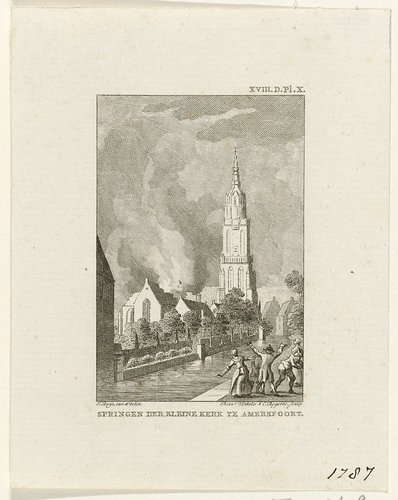
\includegraphics[width=\linewidth]{./Images/Chapter04/example_1.jpg}
\endminipage
\minipage{0.3\textwidth}
  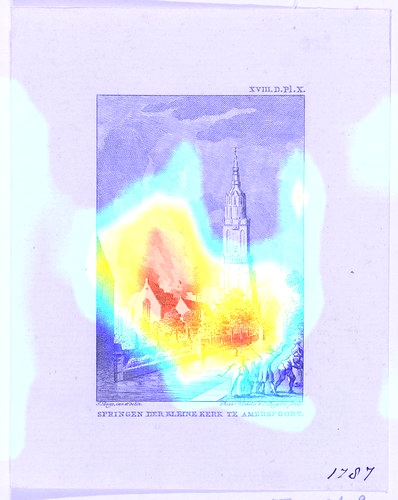
\includegraphics[width=\linewidth]{./Images/Chapter04/imagenet_saliencies_1.jpeg}
\endminipage
\minipage{0.3\textwidth}
  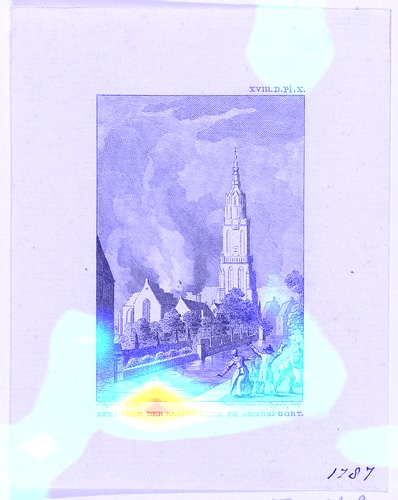
\includegraphics[width=\linewidth]{./Images/Chapter04/rijksnet_saliencies_1.jpeg}
\endminipage

\minipage{0.3\textwidth}
  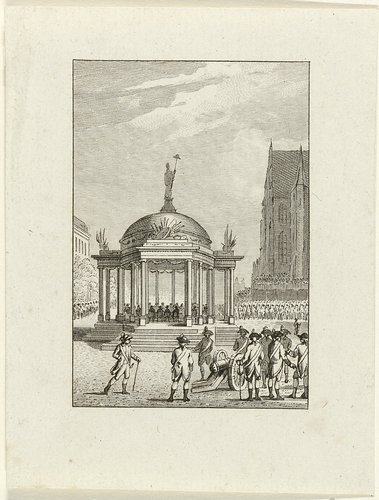
\includegraphics[width=\linewidth]{./Images/Chapter04/example_2.jpg}
\endminipage
\minipage{0.3\textwidth}
  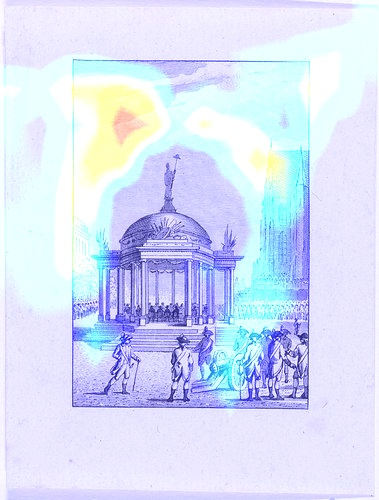
\includegraphics[width=\linewidth]{./Images/Chapter04/imagenet_saliencies_2.jpeg}
\endminipage
\minipage{0.3\textwidth}
  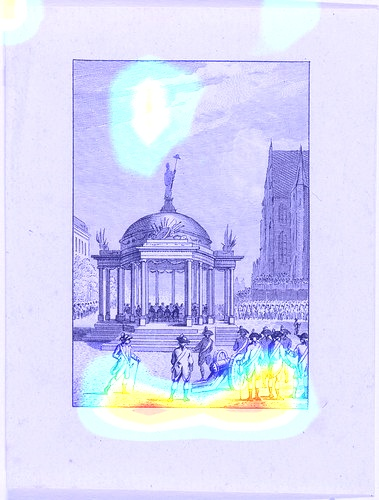
\includegraphics[width=\linewidth]{./Images/Chapter04/rijksnet_saliencies_2.jpeg}
\endminipage

\caption{A visualization of the saliency maps that are obtained when trying to classify an artist of the Rijksmuseum collection (first row of images) with either an ImageNet pre-trained model that is used as simple feature extractor(second row of images), or with the same kind of model which gets fine-tuned (third row of images). We can observe that after getting fine-tuned the network develops novel selective attention mechanisms that allow it to shift its attention from e.g., the buildings depicted in the paintings to the people represented at the bottom.}
\label{fig:saliency_maps}
\end{figure*}


These observations can be related to parallel insights in authorship attribution research \cite{stamatatos:2009}, an established task from Natural Language Processing that is highly similar in nature to artist recognition. In this field, preference is typically given to high-frequency function words (articles, prepositions, particles etc.) over content words (nouns, adjectives, verbs, etc.), because the former are generally considered to be less strongly related to the specific content or topic of a work. As such, function words or stop words lend themselves more easily to attribution across different topics and genres. In art history, strikingly similar views have been expressed by the well-known scholar Giovanni Morelli (1816-1891), who published seminal studies in the field of artist recognition \cite{wollheim:1972}. In Morelli's view too, the attribution of a painting could not happen on the basis of the specific content or composition of a painting, because these items were too strongly influenced by the topic of a painting or the wishes of a patron. Instead, Morelli proposed to base attributions to so-called \emph{Grundformen} or small, seemingly insignificant details that occur frequently in all paintings and typically show clear traces of an artist's individual style, such as ears, hands or feat, a painting's function words, so to speak. The saliency maps above reveal a similar shift in attention when the ImageNet weights are adapted on the Rijksmuseum data: instead of focusing on higher-level content features, the network shifts its attention to lower layers in the network, seemingly focusing on insignificant details, that nevertheless appear crucial to perform artist attribution.


\section{Conclusion} 
\label{sec:ch_4_conclusion}
 
This chapter provides the first insights into the potential that TL can offer for art classification. We have investigated the behavior of convolutional networks which have been pre-trained initially on a very different classification task and shown how their performance can be improved when a fine-tuneing training approach is adopted. Moreover, we have observed that such neural architectures perform better than if they are trained from scratch and that during the fine-tuning stage, they develop new saliency maps that can provide insights about what makes these models outperform the ones that are pre-trained on the ImageNet dataset only. Such saliency maps reflect themselves in the development of new features, which can then be successfully used by the models when classifying heritage objects from different heritage collections. It turns out that the Rijksmuseum fine-tuned models are a better alternative to the same kind of architectures that are pre-trained on ImageNet only and we hope that they will serve the CV community that will deal with similar machine learning problems in the future.

